\chapter{\label{chap:development}Desenvolvimento da Solução}

\todoin[caption={Detalhes}]{Introdução desse capítulo}

\section{\label{section:project-details}Detalhamento do Projeto}
O primeiro passo para dar início ao desenvolvimento deste projeto é obter uma
cópia do projeto \textit{SpelunkBots}, hospedada no \textit{website} de
versionamento de código
\textit{GitHub}\footnote{https://github.com/GET-TUDA-CHOPPA/SpelunkBots}. O
\textit{framework} conta com o código modificado do \textit{Spelunky} e uma
distribuição do \textit{GameMaker Pro 8.0}, utilizada para compilar e gerar o
arquivo executável do jogo.

Conforme detalhado na seção \ref{section:spelunkbots}, o \textit{SpelunkBots}
disponibiliza duas opções de linguagem de programação para realizar o
desenvolvimento dos \textit{bots}: \textit{GML} ou C++. Portanto, a próxima
etapa do projeto é definir a linguagem de programação que vamos utilizar. Para
este projeto, escolhemos a linguagem de programação \textbf{C++}, tendo em vista
que o desenvolvimento utilizando a linguagem \textit{GML} é extremamente
limitado. Além disso, é possível encontrar na Internet algumas bibliotecas em
C++ que implementam a técnica
\textit{NEAT}\footnote{http://nn.cs.utexas.edu/?neat-c}. O uso de uma biblioteca
salva tempo de desenvolvimento e permite que o foco do trabalho seja somente no
desenvolvimento dos \textit{bots}, e não na arquitetura necessária para tal.

Sabendo que a técnica \textit{NEAT} requer que o \textit{bot} receba treinamento
através de diversas simulações do jogo, optamos pelo uso de um servidor
dedicado, pois este processo pode ser demorado e realizá-lo em uma máquina
doméstica -- que está muito mais sujeita a ser desligada acidentalmente ou
intencionalmente -- seria arriscado. O servidor em questão utiliza um sistema
operacional baseado em \textit{Linux}.  Contudo, \textit{Spelunky} foi
desenvolvido utilizando uma versão muito antiga do \textit{GameMaker} e a
compilação do código externo do \textit{SpelunkBots} ocorre através de um
projeto em \textit{Visual Studio}.  Estas ferramentas só podem ser executadas no
sistema operacional \textit{Windows}. Como nosso servidor é baseado em
\textit{Linux}, é necessário realizar algumas adaptações no processo de
compilação e execução. Assim, utilizaremos os \textit{softwares}
\textit{MinGW}\footnote{http://www.mingw.org} e
\textit{Wine}\footnote{https://winehq.org}, que nos permitirão, respectivamente,
compilar o código C++ e gerar a \textit{DLL} e executar programas da plataforma
\textit{Windows} dentro do sistema operacional \textit{Linux}.

O próximo passo é escolher a biblioteca de inteligência artificial da técnica
\textit{NEAT} e incluí-la no processo de compilação da \textit{DLL},
integrando-a ao projeto \textit{SpelunkBots}. Ao concluir este passo, as
configurações iniciais do projeto estarão finalizadas e daremos início ao
processo de modelagem e desenvolvimento dos \textit{bots}. O diagrama
\ref{fig:project-diagram} ilustra a relação entre os elementos de configuração
do projeto.

\begin{figure}[h]
\centering
\begin{tikzpicture}
    \tikzstyle{every node}=[font=\footnotesize, text centered]
    \node (gmm) at (0, 0)  {Game Maker};
    \node (spl) at (0, -2) {Spelunky};
    \node[draw] (spb) at (0, -4) {SpelunkBots};

    \node[text width=4cm] (conf) at (5, 0)  {Configurações \\(escolha do bot e parâmetros de nível)};
    \node (comp) at (5, -4)  {Compilação (MinGW)};

    \node[draw] (neat) at (11, 0) {Biblioteca NEAT};

    \node (dll) at (11, -2) {Solução DLL};

    \node[draw] (bots) at (11, -4) {Código dos \textit{bots}};

    \node at (0, -6) (wine) {Emulação (WineHQ)};

    \node at (5, -6) (linux) {Servidor Linux};

    \node[draw, inner sep=.25cm, fit={(gmm) (spl) (spb)}] (g2) {};
    \node[draw, fit={(spl) (spb)}] {};

    \node[draw, fit={(dll) (bots)}] (g1) {};

    \draw[->, >=latex] (neat.south) -- (g1.north);

    \draw[->, >=latex] (g1.west) -- (comp.east);
    \draw[->, >=latex] (comp.west) -- (spb.east);

    \draw[->, >=latex, in=0, out=200] (conf.west) to (spb.east);

    \draw[->, >=latex] (g2.south) -- (wine.north);
    \draw[->, >=latex] (wine.east) -- (linux.west);
\end{tikzpicture}
\caption {Diagrama do projeto explicando a relação entre os componentes
necessários para o desenvolvimento dos \textit{bots}.
}
\label{fig:project-diagram}
\end{figure}

O \textit{framework} \textit{SpelunkBots} provê uma interface comum para o
desenvolvimento dos \textit{bots} em C++, chamada \textbf{\textit{IBot.h}}. Esta
interface é responsável por expor os métodos e variáveis que os \textit{bots}
utilizam para comunicar-se com o jogo. Portanto, qualquer código de \textit{bot}
desenvolvido deverá partir desta interface. Analisando o arquivo \textit{IBot.h}
é possível perceber que a interface obriga o desenvolvedor a implementar
\textbf{pelo menos} o método \textbf{\textit{Update}}, chamado em todas as
etapas de execução do \textit{bot} para receber informações e enviar comandos ao
jogo. Existem dois outros métodos que podem ser úteis ao desenvolvedor, mas que
não possuem obrigatoriedade de implementação: o \textbf{\textit{Reset}} e o
\textbf{\textit{NewLevel}}. O método \textit{Reset} é chamado no início de todas
as etapas de execução do \textit{bot} para reiniciar suas variáveis de controle.
Este método possui uma implementação padrão que reinicia apenas as variáveis
essenciais (esquerda, direita, pular e atacar). O método \textit{NewLevel} é
chamado toda vez que o \textit{bot} entra em um novo nível, e pode ser usado
para descartar informações do nível anterior sem que seja necessário reiniciar
todas as variáveis do \textit{bot}. Em sua implementação padrão, não executa
nada.

Uma implementação mínima de um \textit{bot} utilizando a interface
\textit{IBot.h} necessitaria, portanto, de dois arquivos: um arquivo
\textit{header}, que conterá as declarações dos métodos e variáveis a serem
utilizadas -- demonstrado no Algoritmo \ref{alg:project-example-bot-header} --,
e um arquivo de implementação -- demonstrado no Algoritmo
\ref{alg:project-example-bot-impl} --, que conterá a implementação das funções
descritas no arquivo \textit{header}.

\section{\label{section:modifications}Modificações Realizadas}

\subsection{\textit{Scripts} de Compilação}

A escolha da linguagem \textit{C++} para a criação dos \textit{bots} requer que
o código seja compilado e que uma \textit{DLL} seja gerada, para que,
posteriormente, seja usada pelo \textit{SpelunkBots}. Este processo é feito em
várias etapas.  Primeiro, compilamos as bibliotecas que utilizamos. Em seguida,
compilamos o código dos \textit{bots} e geramos a \textit{DLL}. Por fim,
movemos a \textit{DLL} para o local onde o \textit{SpelunkBots} será executado.

É necessário executar com sucesso todas as etapas de compilação para viabilizar
o desenvolvimento dos \textit{bots}. De forma a automatizar esse processo,
criamos um \textit{script} -- utilizando \textit{shell script} -- responsável
pelo processo de compilação e movimentação de arquivos.

\subsection{Pular Cena Inicial do Jogo}

O \textit{Spelunky} conta com uma cena inicial, onde o jogador se desloca da
superfície para dentro de uma caverna que permite que ele escolha entre fazer o
tutorial do jogo, iniciar sua aventura ou ver as maiores pontuações. A figura
\ref{fig:spelunky-introduction} apresenta a cena inicial, onde o jogador entra
na caverna de escolha.

\begin{figure}[H]
\centering
	\begin{subfigure}[b]{0.4\textwidth}
		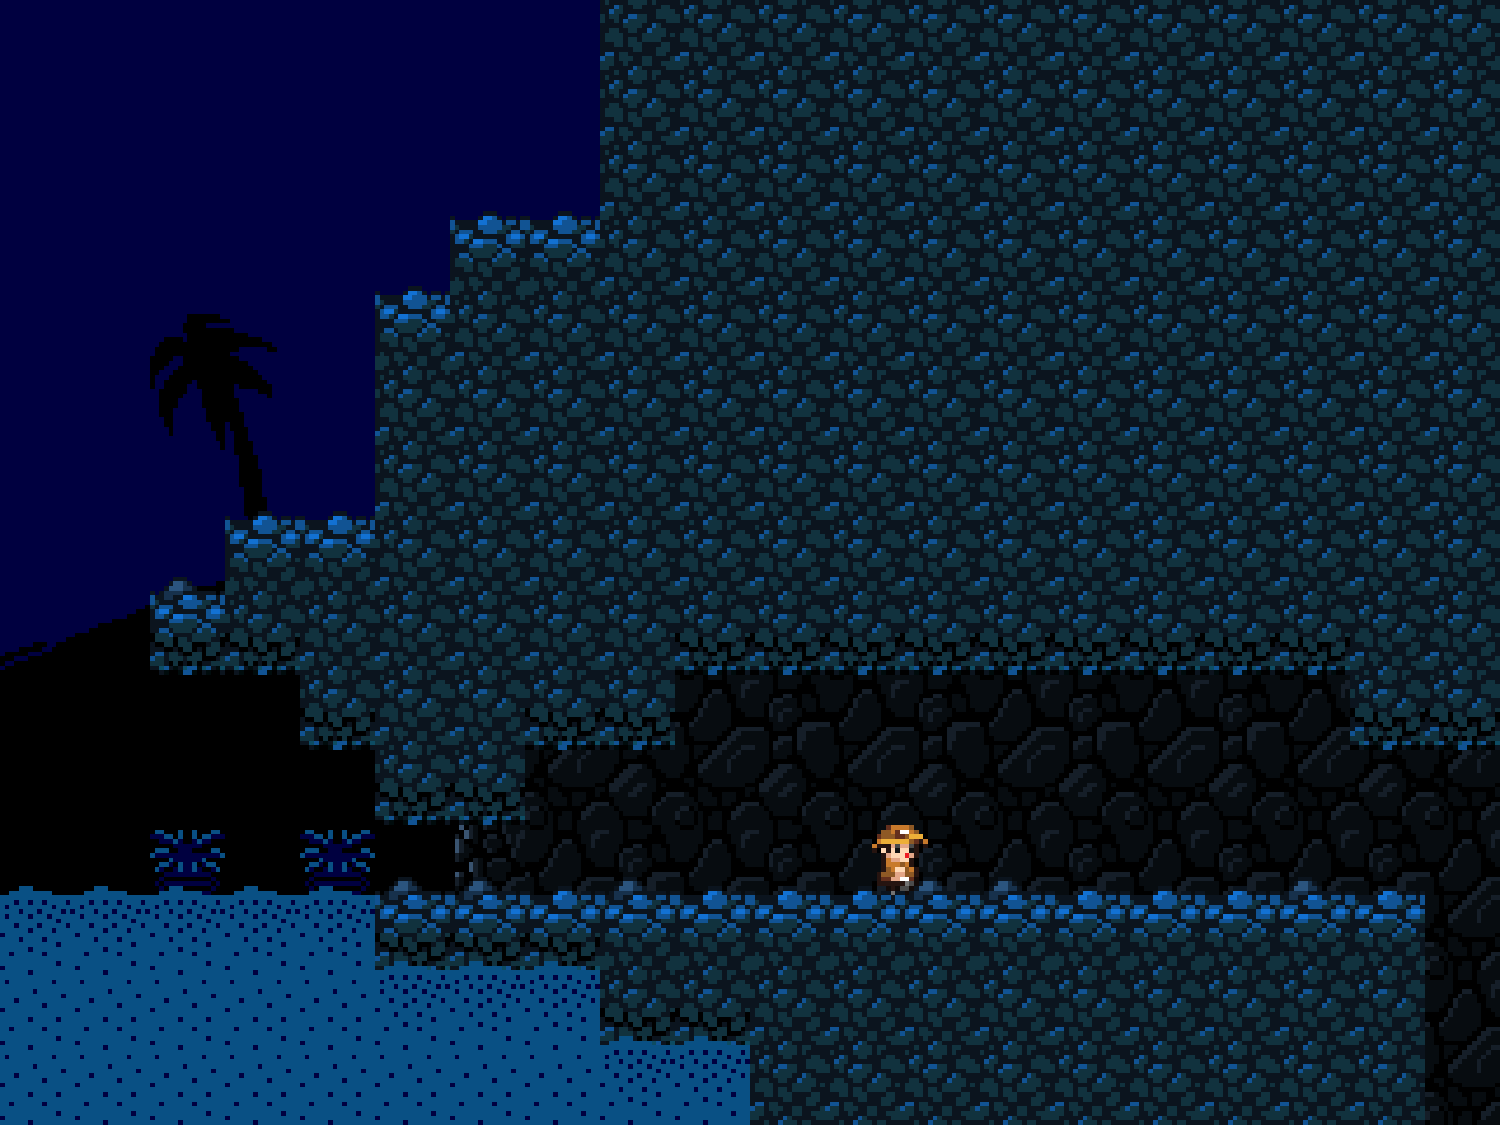
\includegraphics[width=\textwidth]{fig/spelunky-intro-screen.pdf}
		\caption{Entrada para a caverna inicial.}
		\label{fig:spelunky-intro-screen}
	\end{subfigure}
	\begin{subfigure}[b]{0.4\textwidth}
		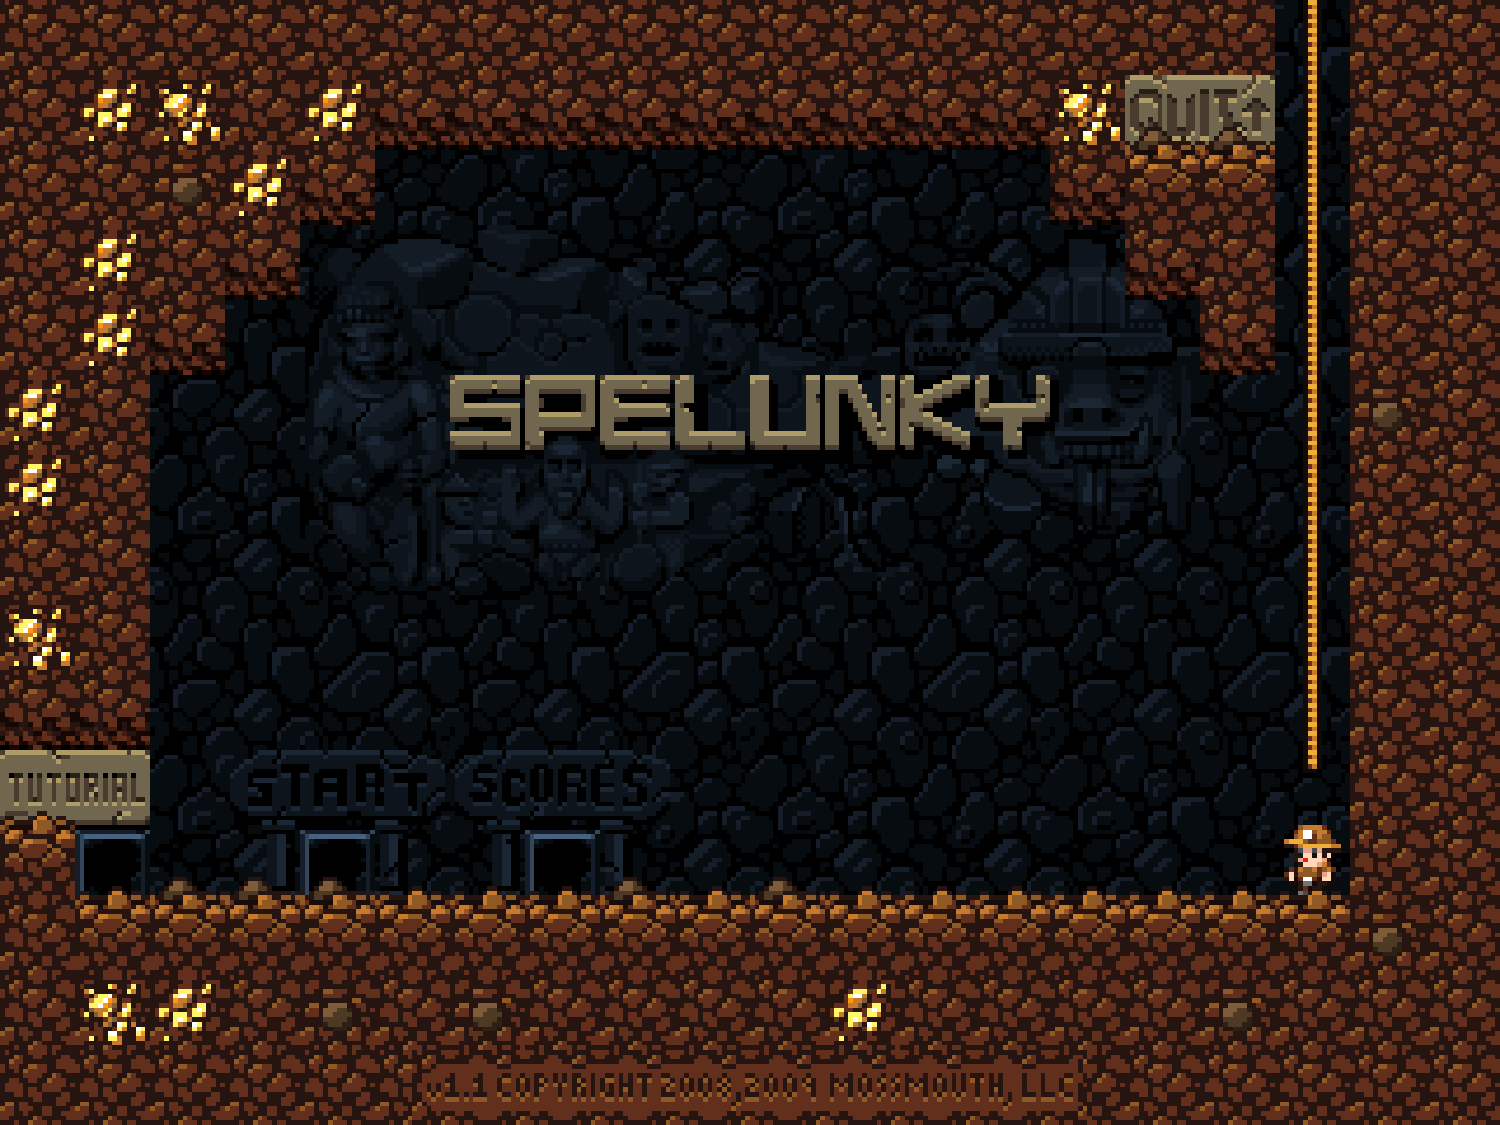
\includegraphics[width=\textwidth]{fig/spelunky-initial-screen.pdf}
		\caption{Caverna de escolha.}
		\label{fig:spelunky-initial-screen}
	\end{subfigure}

    \caption{Cena de introdução do jogo, onde o jogador se desloca da
    superfície para uma caverna com opções de escolha.}
	\label{fig:spelunky-introduction}
\end{figure}

Essas cenas são apenas uma forma de introdução ao jogo, não contribuíndo para a
geração de resultados de execução. Logo, não necessitamos delas. Nossos
\textit{bots} devem ser levados diretamente até a opção de iniciar o jogo.
Assim, utilizamos \textit{GameMaker} para remover essas cenas. Portanto, ao
executar o jogo, o \textit{bot} é levado diretamente ao nível escolhido,
executando imediatamante.

\subsection{Parar a Execução Quando o \textit{Bot} Está Ocioso}

É muito importante conseguirmos definir o momento em que algum \textit{bot}
esteja em um estado não promissor -- gastanto tempo de execução --. Isso
permite que descartemos essa execução, acelerando o processo de treinamento.
Para isso, definimos dois critérios que nos permitem identificar o momento em
que um \textit{bot} está ocioso:

\begin{description}
    \item [Tempo parado] em alguns casos, o \textit{bot} pode escolher ficar
        parado. Porém, caso ele fique parado por muito tempo, é muito provável
        que esteja ocioso. Assim, quando identificamos que o \textit{bot} está
        parado há mais de \textbf{3 segundos}, descartamos sua execução.
    \item [Número de visitas à um mesmo local] caso o \textit{bot} passe pelo
        mesmo local por mais de \textbf{10 vezes}, podemos identificar que ele
        está repetindo suas ações e possivelmente nunca encontrará a porta de
        saída.
\end{description}

Com esses critérios de ociosidade, é necessário que tenhamos uma forma de parar
a execução do \textit{bot} nos casos anteriormente descritos. Assim,
implementamos uma \textbf{verificação de ociosidade}. A cada ciclo de execução
do jogo, verificamos se o \textit{bot} está parado, incrementando um contador
de tempo caso esteja. Zeramos esse contador caso ele se movimente. Após,
incrementamos o contador que indica o número de vezes que o \textit{bot}
visitou a posição em que está. Caso ele esteja parado pelo determinado número
de segundos ou tenha visitado o mesmo estado pelo determinado número de vezes,
sabemos que esse é um estado não promissor. Então, zeramos o número de pontos
de vida dele, fazendo com que o \textit{bot} perca uma vida e passe a executar
novamente.

\subsection{Arquivo de Inicialização}

O processo de escolha das configurações para a execução do jogo requer
experimentação. É necessário combinar diferentes parâmetros e avaliar sua
execução, escolhendo então os parâmetros que produzem os melhores resultados.
No caso do \textit{SpelunkBots}, essa escolha está ligada diretamente à edição
do código do jogo no \textit{Game Maker}. Sempre que desejamos editar um
parâmetro de execução, abrimos o \textit{software}, realizamos a edição dos
valores, salvamos uma nova versão do jogo e então o executamos. Esse processo é
manual e custoso, dificultando a escolha dos melhores parâmetros para execução.  

Dessa forma, alteramos o código do \textit{SpelunkBots} para permitir a leitura
de um arquivo de
inicialização\footnote{https://docs.yoyogames.com/source/dadiospice/002\_reference/file\%20handling/ini\%20files/index.html},
fazendo com que o jogo utilize valores dinâmicos para os parâmetros, sendo
possível então testar novas configurações e alterar a execução do jogo sem
a necessidade de abrirmos o \textit{Game Maker}. Tal arquivo tem um formato
bastante simples, onde cada elemento tem um nome que o identifica e um
valor associado, podendo estar em uma categoria.

O algoritmo ~\ref{alg:ini-file} apresenta esse arquivo de inicialização. Foram
utilizadas quatro categorias de valores. \textit{\textbf{[Bot]}} representa as
informações sobre o \textit{bot} escolhido na execução. A entrada
\textit{bot\_is\_cpp}, quando com o valor \textbf{1}, indica que se trata de um
\textit{bot} que foi escrito em \textit{C++}, já a entrada
\textit{bot\_cpp\_num} idica qual \textit{bot} será executado.  A categoria
\textit{\textbf{[Test]}} informa dados relativos ao teste que será realizado. O
tipo de mapa é informado pela entrada \textit{test\_type}. O parâmetro
\textit{test\_rank} indica ao \textit{SpelunkBots} como classificar a execução
dos \textit{bots}. Podemos controlar o número \textbf{máximo} de execuções pelo
valor de \textit{test\_num}. Também é possível limitar o tempo de vida de um
\textit{bot} pelo parâmetro \textit{test\_time}, que é indicado em segundos.
Podemos especificar os níveis que serão utilizados pelas entradas da categoria
\textit{\textbf{[Levels]}}. Primeiro, indicamos a quantidade de níveis pelo
valor de \textit{level\_num}. Após, para cada nível, indicamos o seu nome em
uma propriedade específica. No caso do primeiro, usamos a propriedade
\textit{level0}, para o segundo, \textit{level1}, e assim para todos eles.  Por
fim, temos a categoria \textit{\textbf{[FAMW]}}, que parametriza a exibição de
informações de depuração durante a execução do jogo.  O valor de
\textit{vision\_debug} indica se deverá ser exibida na tela uma janela da visão
do \textit{bot}, com o tamanho informado por \textit{vision\_size}.

\begin{algorithm}[H]
\lstinputlisting[style=customC++]{code/spelunkbots.ini}
\caption[Arquivo de inicialização de exemplo.]
{\label{alg:ini-file}Arquivo de inicialização de exemplo.}
\end{algorithm}

\subsection{\label{sub:virtual-display}Execução com Display Virtual}

O servidor \textit{Linux} que utilizamos para a execução não possui nenhuma
interface gráfica, além disso, não existe uma forma de executar o
\textit{Spelunky} ou o \textit{SpelunkBots} sem considerar uso de uma.

Porém, é possível fazer a criação de um \textit{display} virtual, onde
simulamos uma interface gráfica semelhante a uma real. Nesse caso, fizemos o
uso do
\textit{XVFB}\footnote{https://www.x.org/archive/X11R7.6/doc/man/man1/Xvfb.1.xhtml},
criando então uma interface gráfica que recebe a execução do jogo. O uso de uma
interface gráfica virtual também nos permite que gravemos vídeos do jogo, além
de permitir a captura de imagens da tela, permitindo que depuremos a execução
do jogo.

\section{\label{section:neat-details}Implementação do NEAT}

\todoin[caption={Implementação do NEAT}] {
    Explicar itens como:

    \begin{itemize}
		\item Lib utilizada
        \item Rede neural inicial
            \item Ferramenta para geração da rede inicial
        \item Parâmetros do NEAT
        \item Armazenamento dos resultados obtidos
        \item Explicação de cada um dos arquivos do NEAT (NEATBot.h, NEATOutput.h, NEATBotViewer, etc.)
    \end{itemize}
}

